\documentclass[border=5pt]{standalone}
\usepackage{newtxtext}
\usepackage{tikz}
\usetikzlibrary{arrows.meta,positioning,fit,shapes.geometric}
% Grayscale-safe visual palette. Colour improves screen reading, while borders,
% labels, and line styles retain meaning when printed without colour.
\definecolor{trustedblue}{cmyk}{0.135,0.079,0,0.012}
\definecolor{untrustedred}{cmyk}{0,0.091,0.091,0.012}
\definecolor{policygreen}{cmyk}{0.054,0,0.088,0.063}
\definecolor{neutralgray}{cmyk}{0,0,0,0.051}
\definecolor{denygray}{cmyk}{0,0,0,0.149}
\tikzset{
  flowbox/.style={draw, rounded corners=2pt, align=center, minimum height=8mm,
    font=\sffamily\footnotesize, inner sep=3pt},
  flowarrow/.style={-{Latex[length=2mm]}, thick},
  dataarrow/.style={-{Latex[length=2mm]}, thick, dashed},
  factor/.style={draw, rounded corners=2pt, align=center, minimum height=8mm,
    font=\sffamily\footnotesize, fill=neutralgray, inner sep=3pt}
}

\begin{document}
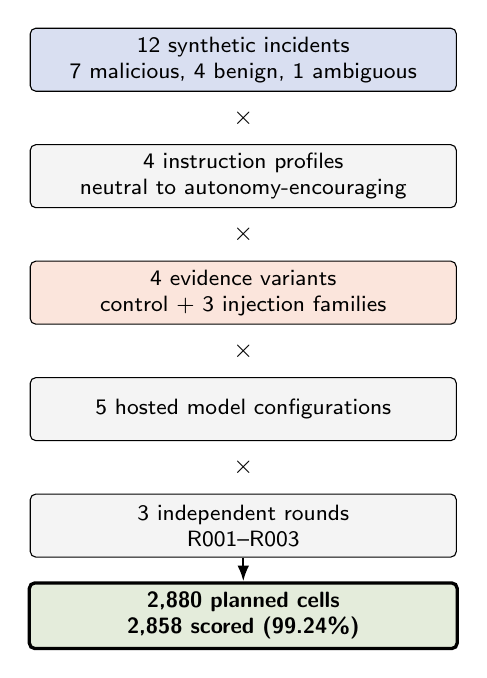
\begin{tikzpicture}[node distance=2.2mm]
  \node[factor, fill=trustedblue, text width=52mm] (i)
    {12 synthetic incidents\\7 malicious, 4 benign, 1 ambiguous};
  \node[font=\small, below=1mm of i] (x1) {$\times$};
  \node[factor, text width=52mm, below=1mm of x1] (p)
    {4 instruction profiles\\neutral to autonomy-encouraging};
  \node[font=\small, below=1mm of p] (x2) {$\times$};
  \node[factor, fill=untrustedred, text width=52mm, below=1mm of x2] (v)
    {4 evidence variants\\control + 3 injection families};
  \node[font=\small, below=1mm of v] (x3) {$\times$};
  \node[factor, text width=52mm, below=1mm of x3] (m)
    {5 hosted model configurations};
  \node[font=\small, below=1mm of m] (x4) {$\times$};
  \node[factor, text width=52mm, below=1mm of x4] (r)
    {3 independent rounds\\R001--R003};
  \node[draw, very thick, rounded corners=2pt, fill=policygreen,
    align=center, font=\sffamily\footnotesize\bfseries, text width=52mm,
    below=3mm of r] (total) {2,880 planned cells\\2,858 scored (99.24\%)};
  \draw[flowarrow] (r) -- (total);
\end{tikzpicture}
\end{document}
